\documentclass{beamer}
\usetheme[sectionpage=none, progressbar=frametitle, numbering=none]{metropolis}        % Use metropolis theme
\usepackage{tikz}
\usepackage{fixltx2e}
\usetikzlibrary{tikzmark,decorations.pathreplacing,calc}
\usepackage{listings}
\setbeamertemplate{footnote}{%
	\parindent 0em\noindent%
	\raggedright
	\usebeamercolor{footnote}\hbox to 0.6em{\hfil\insertfootnotemark}\insertfootnotetext\par\hfil%
	}
\title{An Architecture for Steering Traffic and Computations
via Deep Learning in Challenged Edge Networks}
% \date{\today}
\date{October 11\textsuperscript{th}, 2019}
%\date{February 16, 2018}
\author{Alessandro Gaballo, Matteo Flocco, Flavio Esposito, Guido Marchetto}
\institute{Saint Louis University, Politecnico di Torino\par~\\~\\~\\~\\~\\~\\~\\~\\~\\~\\\tiny{\textit{Invited Paper}}}
\setbeamertemplate{frametitle continuation}{\insertcontinuationcount}
% logo of my university
\titlegraphic{%
  \begin{picture}(0,0)
	\put(310,-150){\makebox(0,0)[rt]{\includegraphics[width=2.cm]{img/slu_logo}}
	}
  \end{picture}
  \begin{picture}(0,0)
	\put(230,-155){\makebox(0,0)[rt]{\includegraphics[width=2.cm]{img/politologo}}
	}
  \end{picture}} 
\AtBeginSection[]{
%\frame{\sectionpage}
}

\newcommand{\mytoc}{\frame{\frametitle{Talk overview}\tableofcontents[currentsection,currentsubsection,subsectionstyle=show/shaded/hide, subsubsectionstyle=show/shaded/hide]}}



%subsubsection page
\newcommand{\subsubsectionpage}{
\begin{frame}
  \centering
  \begin{minipage}{22em}
    \raggedright
    \usebeamercolor[fg]{section title}
    \usebeamerfont{section title}
    \insertsectionhead\\[-1ex]
    \usebeamertemplate*{progress bar in section page}
    \par
    \ifx\insertsubsectionhead\@empty\else%
      \usebeamercolor[fg]{subsection title}%
      \usebeamerfont{subsection title}%
      \insertsubsectionhead{} -- \insertsubsubsectionhead
    \fi
  \end{minipage}
  \par
  \vspace{\baselineskip}
\end{frame}
}

\newcommand\blfootnote[1]{%
  \begingroup
  \renewcommand\thefootnote{}\footnote{#1}%
  \addtocounter{footnote}{-1}%
  \endgroup
}

% reshaping list circles bullet
\setbeamertemplate{section in toc}{\leavevmode\leftskip=2ex%
  \llap{%
    \usebeamerfont*{section number projected}%
    \usebeamercolor{section number projected}%
    \begin{pgfpicture}{-1ex}{0ex}{1ex}{2ex}
      \color{bg}
      \pgfpathcircle{\pgfpoint{0pt}{.75ex}}{.6ex}
      \pgfusepath{fill}
      %\pgftext[base]{\color{fg}\inserttocsectionnumber}
    \end{pgfpicture}\kern1.25ex%
  }%
  \inserttocsection\par}
  
\setbeamertemplate{subsection in toc}{\leavevmode\leftskip=1em$\bullet$\hskip1em\inserttocsubsection\par}
\setbeamertemplate{subsubsection in toc}{\leavevmode\leftskip=3em$\bullet$\hskip1em\inserttocsubsubsection\par}

%temporary until I remake the imgs
\setbeamercolor{background canvas}{bg=white}

\definecolor{colori}{RGB}{166,35,41}
\definecolor{colorii}{RGB}{248,219,162}

\NewDocumentCommand\MyArrow{O{0pt}mmmO{out=150,in=210}}
{%
\begin{tikzpicture}[overlay, remember picture]
  \draw [->,thick,line width=4pt,#4]
    ( $ ({pic cs:#3}|-{pic cs:#2}) + (-#1,1.3ex) $ ) to[#5]  
    ( $ (pic cs:#3) + (-#1,0) $ );
\end{tikzpicture}%
}

\begin{document}
\maketitle
\section*{Motivation}
  \begin{frame}{How many times have you delegated a task?}
	\includegraphics[width=\textwidth]{img/delegation.pdf}  
  \end{frame}
  
  \frame{\frametitle{What is task offloading?}
  	\begin{columns}[totalwidth=\textwidth]
	\begin{column}{0.65\textwidth}
	  Task offloading is the process of transferring tasks to another platform. \\~\\
  It is often adopted in the context of Mobile Edge Computing (MEC). \\~\\
  The goal is to reduce power consumption and get results faster.
	\end{column}
	\begin{column}{0.33\textwidth}  %%<--- here
	\centering	
	\includegraphics[scale=0.4]{img/offloading.pdf}
	\end{column}
	\end{columns}

  }
   \frame{\frametitle{How should tasks be offloaded?}
	There is no architecture describing the offloading mechanisms.\\~\\
	Currently used routing strategies, such as OSPF, are performance unaware.\\~\\OSPF computes the shortest path to a destination, without considering any performance indicator, which can be crucial in critical scenarios.
  }  
  
  \frame{\frametitle{What tools do we have?}
	Recently Software-Defined Networking (SDN) has spreaded, with the idea of separating data and control plane. \\~\\
	Knowledge-Defined Networking (KDN) is the idea of building a knowledge plane~(1) for the network and manage it accordingly.\\~\\
	The combination of SDN \& KDN is a powerful tool for network management.\\~\\~\\
	 \begin{columns}[totalwidth=\textwidth]
	\begin{column}{0.35\textwidth}
	~
	\end{column}
	\begin{column}{0.63\textwidth}  %%<--- here
	
	\scriptsize{[1] D. Clark, C. Partridge, J. Ramming, and J. Wroclawski. \\
	\textbf{A knowledge plane for the internet.} \\
	In Proc. of SIGCOMM '03. ACM, New York, NY, USA, 3-10.}
	\end{column}
	\end{columns}
  }
  
  \begin{frame}{What can we do?}
	\begin{itemize}
		\item Architecture definition to address the complexity problem
		\item Knowledge Plane to support network management
		\item Performance aware traffic steering
	\end{itemize}
  \end{frame}
  \begin{frame}{Talk overview}
	\tableofcontents[hideallsubsections]
  \end{frame}
\section{Offloading Architecture}
\subsection{Architecture}
	\mytoc
	\frame{\frametitle{What is an architecture?}
	In Computer Science and Engineering, an architecture describes the necessary and sufficient set of invariances to achieve a goal. \\~\\The architecture is also responsible of separating the different functionalities by identifying who does what.}
	\begin{frame}{Our contribution: offloading architecture}
		\centering
		\includegraphics[scale=0.5]{img/off_sys_arch.pdf}
	\end{frame}
\subsection{Task Offloading Protocol}
	\mytoc
	\begin{frame}{Our contribution: task offloading protocol}
		\centering
		\includegraphics[scale=0.3]{img/protocol_sequence.pdf}
		\flushleft
		The protocol allows the client to specify:
		\begin{itemize}
		\item task requirements such as CPU, memory and latency
		\item offloading logic (e.g. nearest server)
		\end{itemize}
	\end{frame}
\subsection{Path Prediction via Deep Learning}	
\subsubsection{Overview}
	\mytoc
	\begin{frame}{Our contribution: path prediction via deep learning}
	Machine learning is a powerful tool for inference tasks
	\\~\\
	\centering	
	{\Huge$\Downarrow$}
	\flushleft
	\textbf{IDEA:} Routing problem as inference problem
	\end{frame}
	\frame{\frametitle{How to determine the best path?}Use traffic pattern as performance indicator.\\Perform path prediction with machine learning.\\~\\	
\centering
	\includegraphics[width=\textwidth]{img/dnn.pdf}	
	}	
	\frame{\frametitle{Long Short-Term Memory (LSTM)}
	LSTM is an evolution of recurrent neural networks (RNNs) capable of memorizing data temporal patterns\\~\\
	\textbf{Objective:}\\Learn how traffic patterns evolve and route accordingly
	}
	\frame{\frametitle{Learning from who?}LSTM RNNs  are a supervised learning method, they require data to learn from.\\ 
	We use OSPF routing decisions as a ground truth.\\~\\
	\centering
	\includegraphics[width=\textwidth]{img/problem_model}
	}
	\frame{\frametitle{Our prediction model}	
	To use a LSTM we must define the model input and output.\\
	~\\
	\begin{columns}[totalwidth=\textwidth]
	\begin{column}{0.49\textwidth}
	\textbf{Input:}\\~\\
	Incoming packets count \\on each router\\~\\
	\end{column}
	\begin{column}{0.49\textwidth}  %%<--- here
	\textbf{Output:}\\~\\
	One-hot encoded vector \\with the next hop in the path\\~\\
\end{column}
\end{columns}
	\centering
	\includegraphics[width=\textwidth]{img/prediction_flow}
	}
	\frame{\frametitle{Path prediction process}Training a single model for all the targets in the topology is not feasible.\\~\\
	\textbf{SOLUTION}: train a model for all the source-destination pairs in the network.\\~\\
	To compute the whole path we iteratively use the model of the predicted next hop until the destination is reached.}
	\frame{\frametitle{Example: computing the path from R1 to R4 }	
	\includegraphics[width=\textwidth]{img/example.pdf}\\
	Step 1 - model = R1-R4 --> next hop = R2\\
	Step 2 - model = R2-R4 --> next hop = R3\\
	Step 3 - model = R3-R4 --> next hop = R4 \\~\\
	Computed path: R1 - R2 - R3 - R4\\}
	\subsubsection{Dataset}
	\mytoc
	\frame{\frametitle{Dataset generation}
	To train our model we need:
	\begin{itemize}
	\item network topology
	\item routing algorithm
	\item packet counter
\end{itemize}
	We could not find any public dataset suited to our needs so we create our own.
	}
	\frame{\frametitle{Network topology}
	We create this topology using MiniNeXt
	\includegraphics[width=\textwidth]{img/network_arch}\\ 
	\tiny{\textit{* All switches are connected to the SDN controller}}	
	}
	\frame{\frametitle{Routing algorithm}
	To run routing algorithms on MiniNeXt nodes we use Quagga.\\
	Quagga is a routing suite providing different routing algorithms (e.g OSPF, IS-IS, RIP).\\~\\
	We choose Open Shortest Path First (OSPF) because of its wide adoption as iBGP.\\
	}
	\frame{\frametitle{Packet counter}
	The SDN controller --Ryu-- is responsible of retrieving the packet count.\\~\\
	\includegraphics[width=\textwidth]{img/packet_counter.pdf}
	}
		
	\frame{\frametitle{Dataset generation steps}
		%\MyArrow[1.3em]{start}{end}{line width=1pt}[out=150, in=210]	
	For an arbitrary number of times:
	\begin{enumerate}
	\item\label{p1} Initialize the topology with different link speed
	\item Simulate traffic between routers
	\item Save packet count and routing tables
	\item Stop the traffic simulation and tear down the network
	\item Back to step~\ref{p1}
	% ADD ARROW FROM THE LAST TO THE FIRST BULLET
	\end{enumerate}
	}
	
%	\subsubsection{LSTM Architecture}
%	\mytoc
%	\frame{\frametitle{How to decide the LSTM structure?}
%	The number of layers and neurons cannot be decided a priori.
%	Cross validation is a powerful technique to determine the model parameters.\\~\\
%	\includegraphics[width=\textwidth]{img/cross_validation}
%	}
%	\frame{\frametitle{Accuracy: more neurons or more layers?}
%	Neurons affect performance more than hidden layers\\~\\	
%	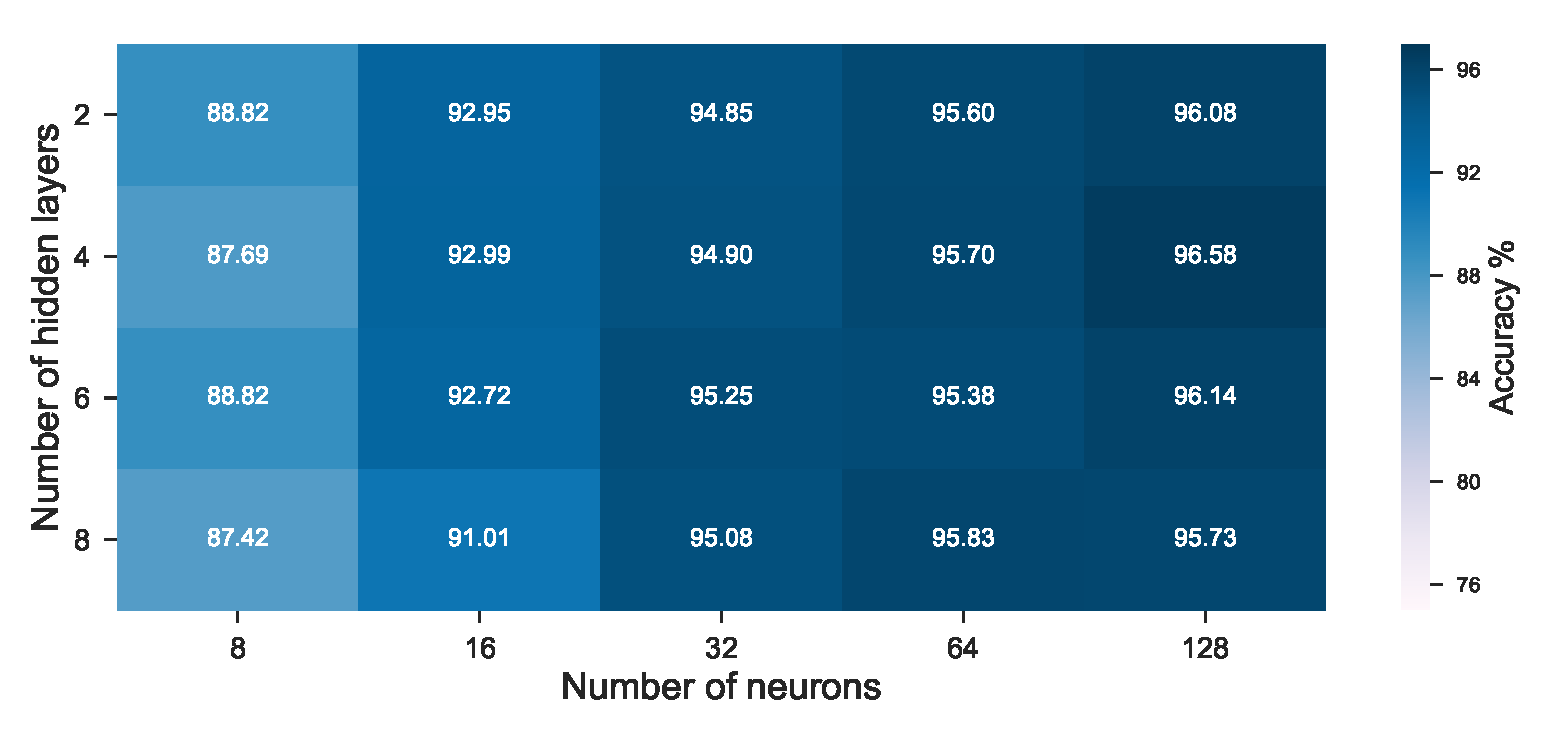
\includegraphics[width=\textwidth]{img/architecture_cmp}	
%	}
%	
%	\frame{\frametitle{Finding the trade-off: training time}
%	\includegraphics[width=\textwidth]{img/timing_cmp}	\\~\\
%	\tiny{\textit{* Accuracy shown only for models with 128 neurons}}	
%	}
%	\frame{\frametitle{Tuning the network: input normalization}
%	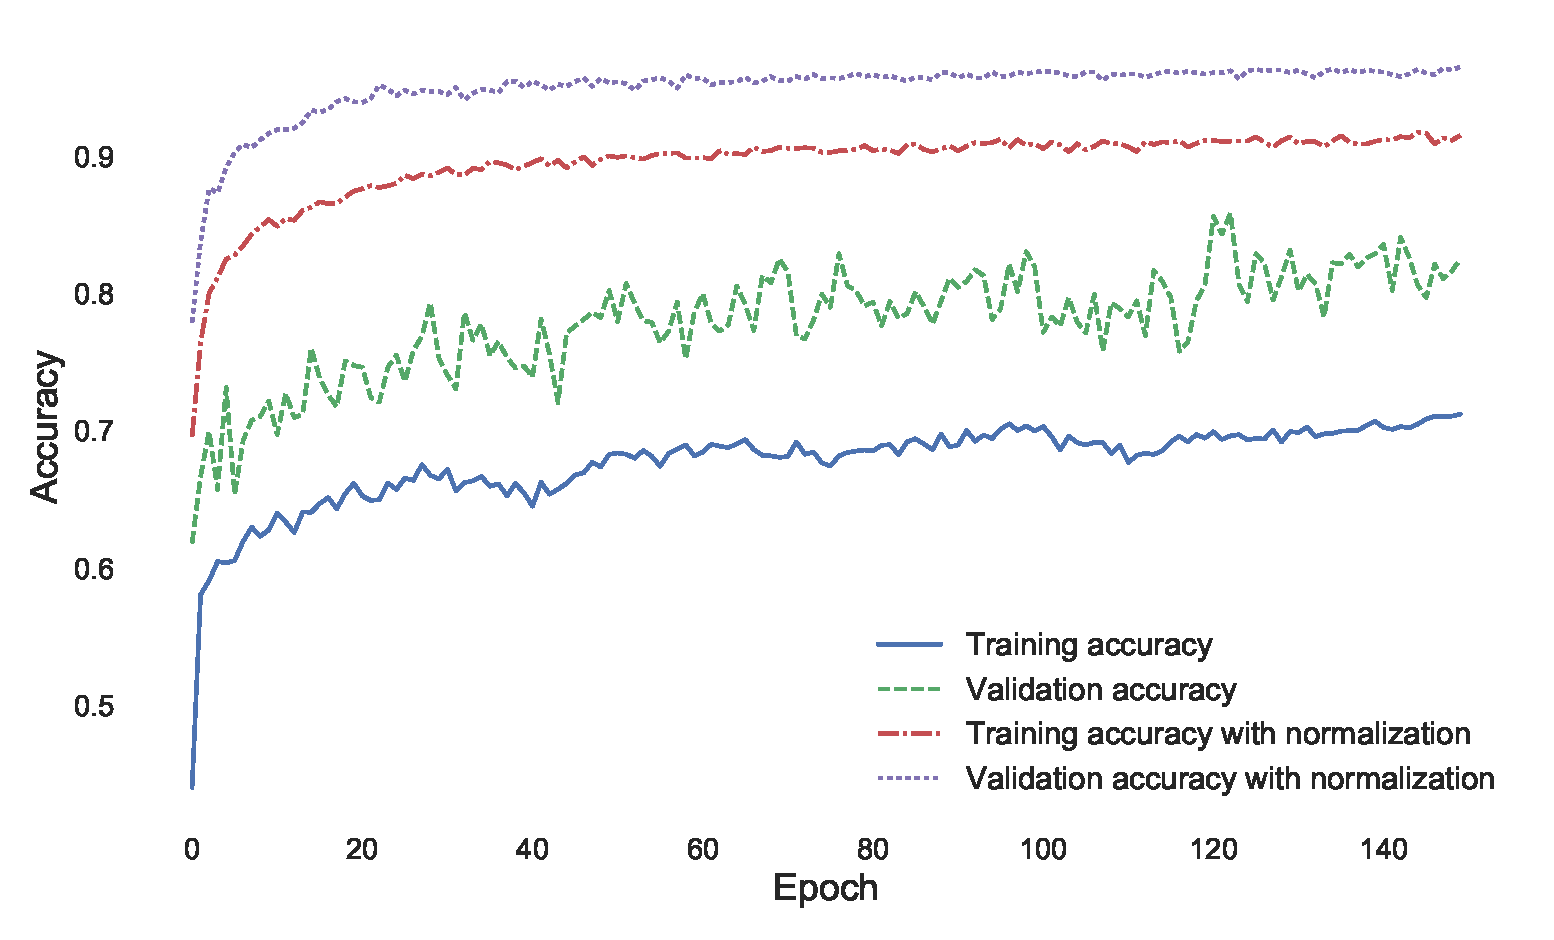
\includegraphics[width=\textwidth]{img/normalization_acc_cmp}	\\~\\
%	\tiny{\textit{* Accuracy shown only for models with 128 neurons}}	
%	}
	


\section{Results}
	\subsection{LSTM architecture}
	\mytoc

	\frame{\frametitle{How to decide the LSTM structure?}
	The number of layers and neurons cannot be decided a priori.
	Cross validation is a powerful technique to determine the model parameters.\\~\\
	\includegraphics[width=\textwidth]{img/cross_validation.pdf}
	}
	\frame{\frametitle{Accuracy: more neurons or more layers?}
	Neurons affect performance more than hidden layers\\~\\	
	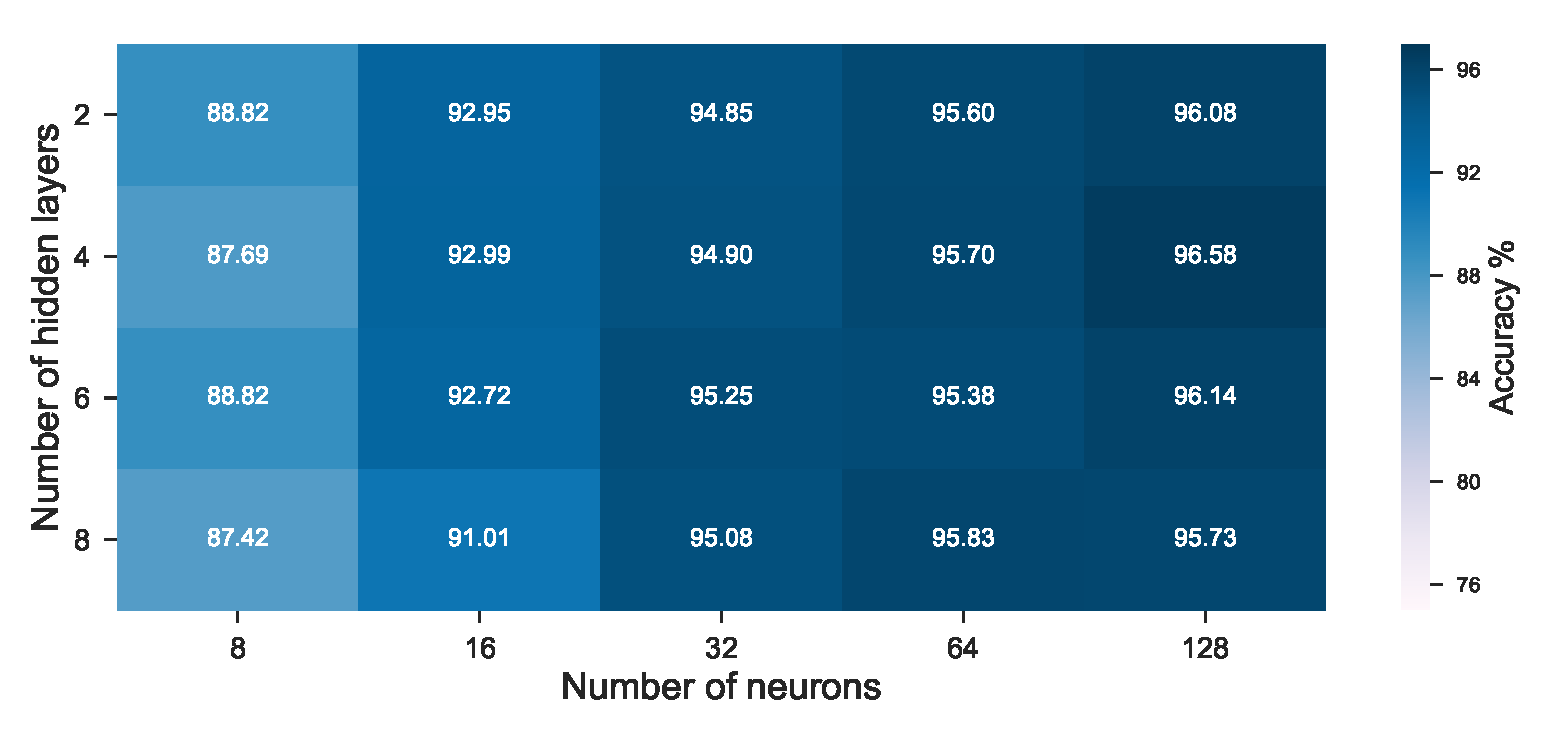
\includegraphics[width=\textwidth]{img/architecture_cmp}	
	}
	
	\frame{\frametitle{Finding the trade-off: training time}
	\includegraphics[width=\textwidth]{img/timing_cmp}	\\~\\
	\tiny{\textit{* Accuracy shown only for models with 128 neurons}}	
	}
	\frame{\frametitle{Tuning the network: input normalization}
	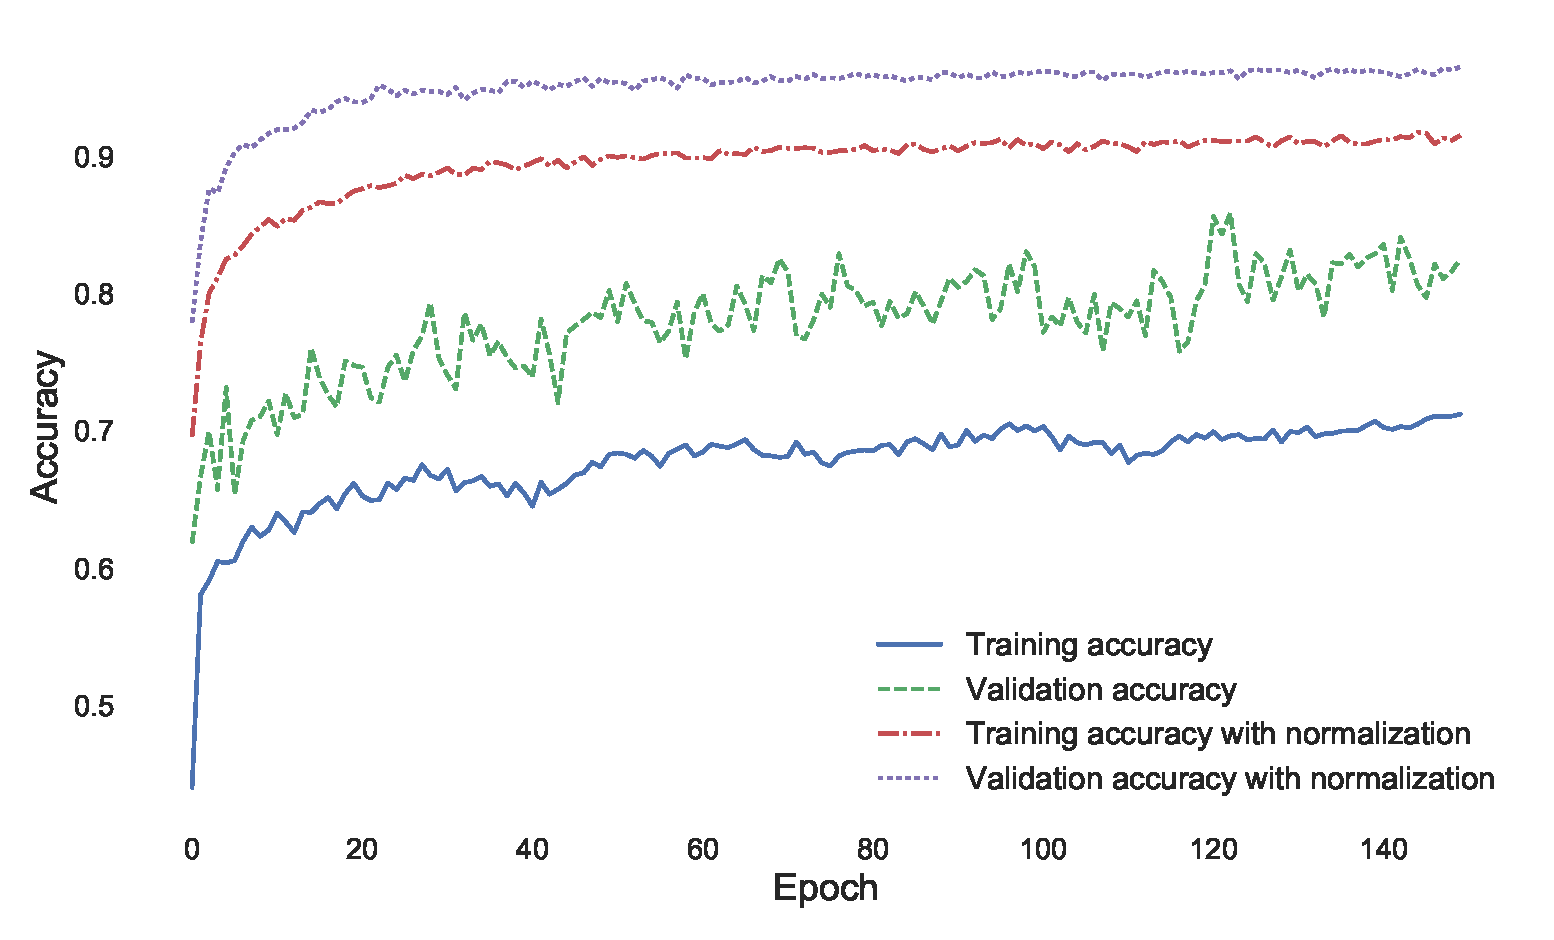
\includegraphics[width=\textwidth]{img/normalization_acc_cmp}	\\~\\
	\tiny{\textit{* Accuracy shown only for models with 128 neurons}}	
	}	
	
	\subsection{Emulating OSPF}
	\mytoc
	\frame{\frametitle{The system is able to emulate OSPF}
	We test the system's ability to behave like OSPF by averaging the performance of all the models on the test set.\\~\\The LSTM achieves an average accuracy of \textbf{98.71\%} with respect to OSPF.}

	\subsection{Performance aware routing}
	\mytoc
	\frame{\frametitle{Is the system performance aware?}
	%We want to investigate the system ability to detect and adapt to network anomalies.\\
	We select a target and analyze, through an example, how our system behaves differently from OSPF in case of link loss.\\~\\
	\centering
	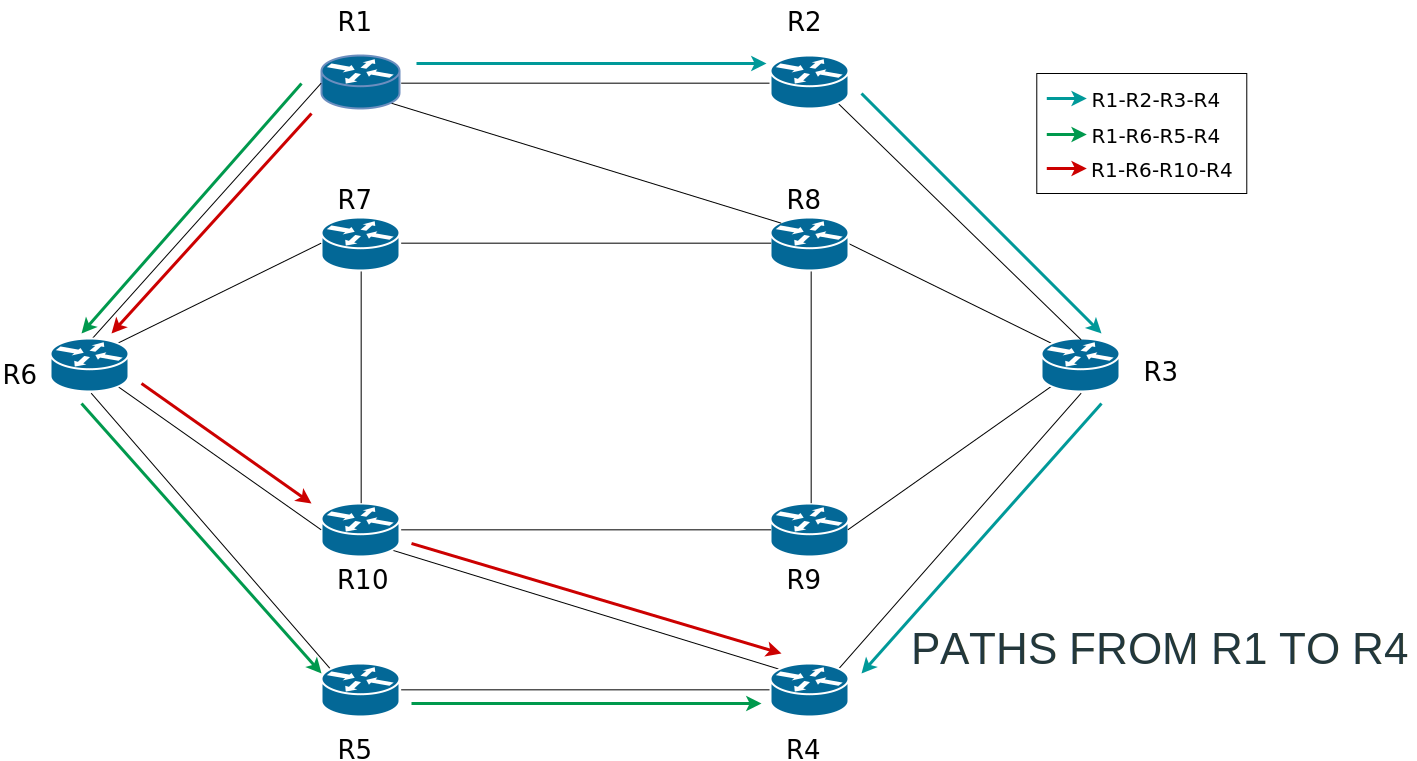
\includegraphics[scale=0.19]{img/validation_target}
	}
	\frame{\frametitle{The system exhibits a dynamic behavior}
	The LSTM path predictor is able to suggest multiple paths\\~\\
	\includegraphics[width=\textwidth]{img/path_comparison}	
	}
	\frame{\frametitle{LSTMs outrun current approaches in terms of retransmission}
	In case of malfunctioning links, our system has a lower retransmission percentage then traditional routing\\~\\
	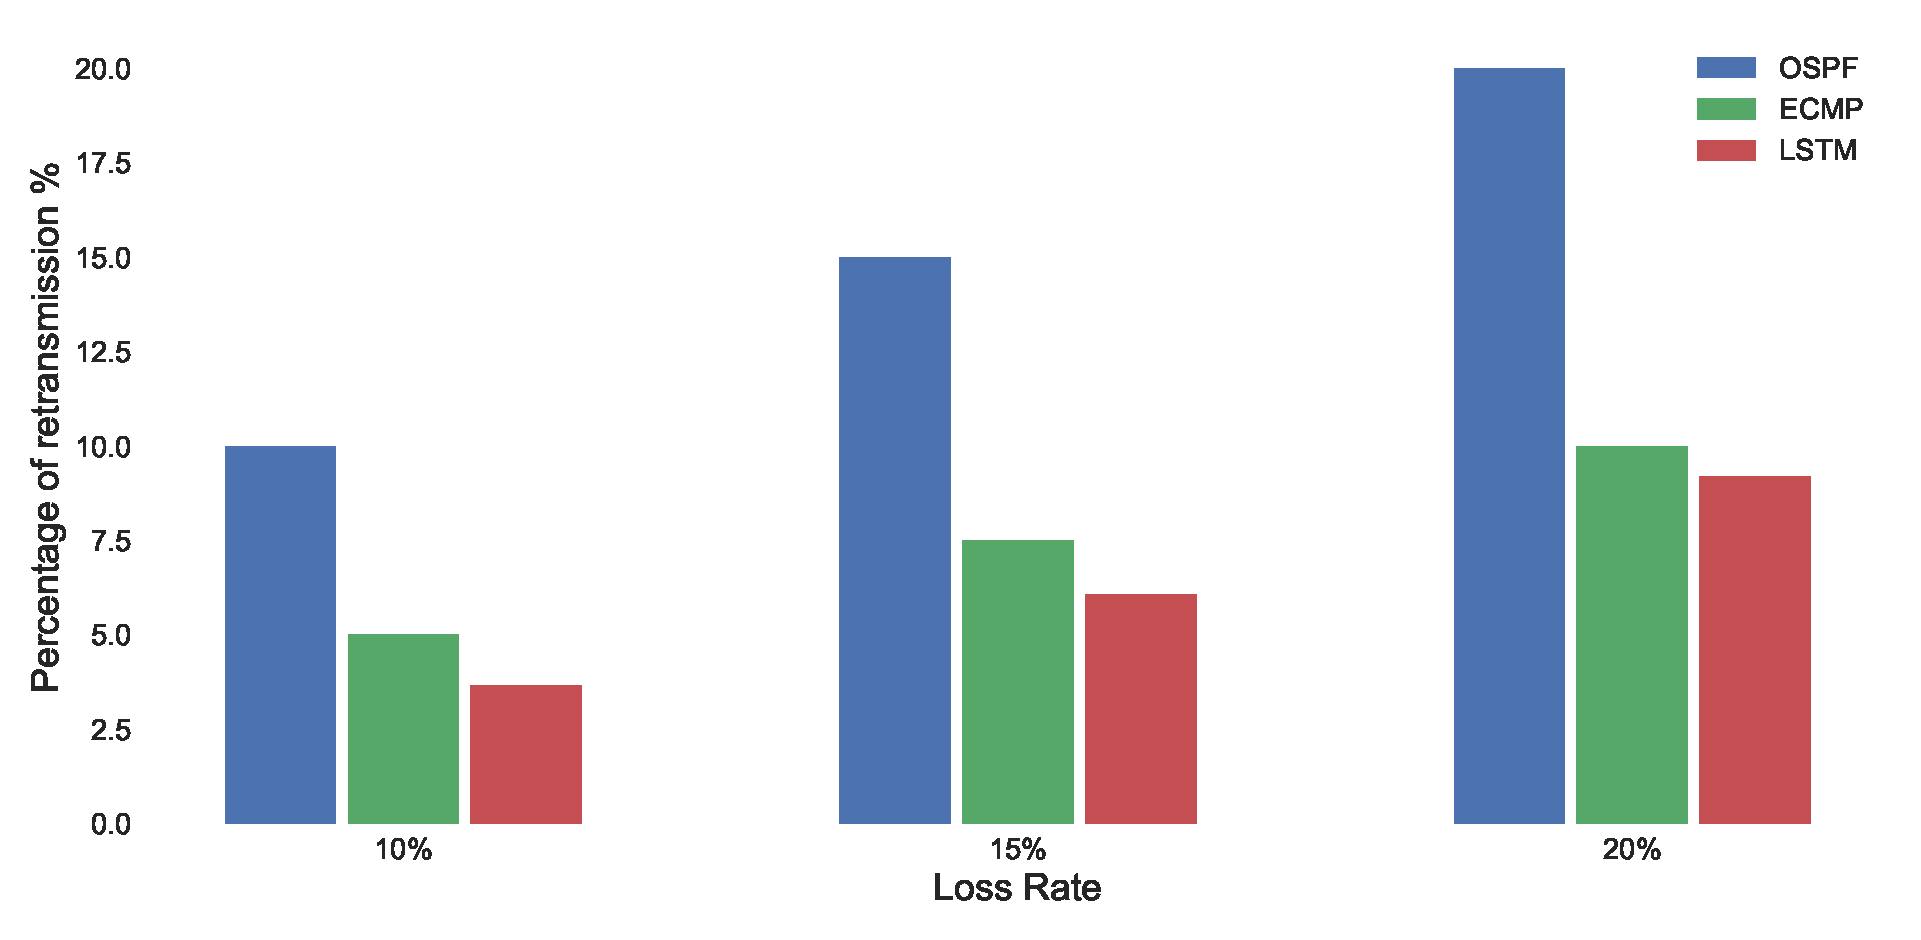
\includegraphics[width=\textwidth]{img/prediction_cmp_bar}\\
	\tiny{\textit{OSPF = Open Shortest-Path First, LSTM = Long Short-Term Memory
}	}}

\section{Limitations}
	\mytoc
	\begin{frame}{Limitations}
	Testbed:
	\begin{itemize}
	\item The functionalities of Mininet are limited
	\item Higher link loss decreases the prediction efficiency
	\end{itemize}
	~\\
	Computation:	
	\begin{itemize}
	\item The number of models to train is big
	\item The trained models occupy GBs of memory
	\end{itemize}
	\end{frame}
	\frame{\frametitle{Future work}
	Current results are encouraging, therefore  we want to further investigate the problem by:
	\begin{itemize}
	\item getting rid of Mininet emulation environment constraints  
	\item testing the method on larger networks (e.g GENI)
	\item running the testbed on a more scalable platform (e.g GPU)
	\item exploring more machine learning techniques \\(e.g reinforcement learning)
\end{itemize}		
	}
\section*{Take home messages}
\begin{frame}{Take home messages}
\begin{itemize}
\item	Mobile edge computing is a complex problem\\
\pause
\item	We prototyped an architecture for MEC offloading orchestration\\
\pause
\item	We developed a machine learning-based, performance aware routing strategy that improves on classic iBGP mechanisms
\end{itemize}	
\end{frame} 

\begin{frame}[standout]
  \Large An Architecture for Task and Traffic Offloading \\in Edge Computing via Deep Learning\\
    \vspace{1cm}
	\large Thank you for the attention\\  
  \vspace{1cm}
  {\small Alessandro Gaballo}
\end{frame}

%backup slides
%backup slides
\begin{frame}[allowframebreaks, noframenumbering, fragile]{Protocol}
\centering
%\textbf{messages.proto}
\begin{lstlisting}
message OffloadRequest {
    message Requirements {
        enum Latency {
            URGENT = 0;
            STANDARD = 1;
            LOOSE = 2;
        }

        float cpu = 1;
        int32 memory = 2;
        Latency latency = 3;
    }
    
    enum Type {
        LAMBDA = 0;
        STANDARD = 1;
    }

    message Task {
        message TaskWrapper {
            enum WrapperType {
                JAR = 0;
                EGG = 1;
            }

            string name = 1;
            WrapperType type = 2;
            bytes task = 3;
        }

        oneof task_location {
            string task_id = 1;
            TaskWrapper wrapper = 2;
        }
    }




    Requirements requirements = 1;
    Type type = 2;
    Task task = 3;

}

message Response{
    enum Result {
        OK = 0;
        INVALID_MSG_SIZE = 1;
        INVALID_REQUEST = 2;
    }

    Result result = 1;
    string msg = 2;
}

message Message{
    enum Type {
        OFFLOAD_REQUEST = 0;
        RESPONSE = 1;
        TASK = 2;
    }
    
    

    Type type = 1;
    oneof msg_type {
        OffloadRequest off_req = 2;
        OffloadRequest.Task task = 3;
        Response response = 4;
    }
}

\end{lstlisting}
\end{frame}

\begin{frame}[noframenumbering]{Recurrent Neural Network vs Long Short Term Memory}
\centering
\includegraphics[width=0.8\textwidth]{img/simple_rnn}\\~\\
\includegraphics[width=0.8\textwidth]{img/simple_lstm}
\end{frame}
\begin{frame}[noframenumbering]{LSTM cells - activation function}
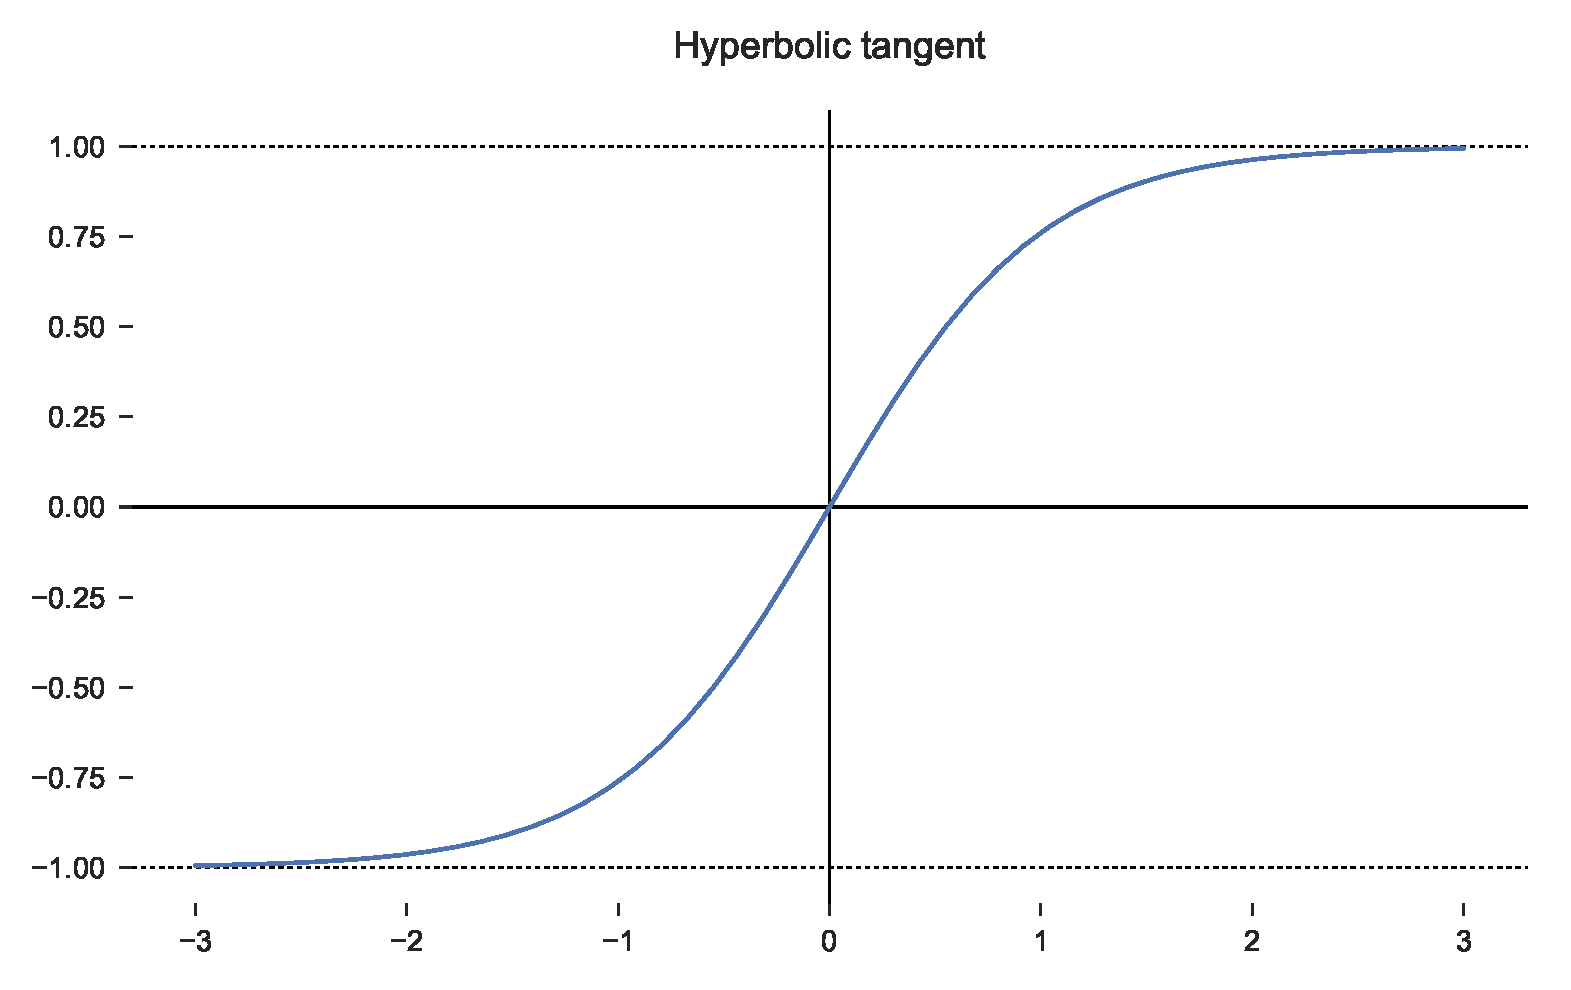
\includegraphics[width=\textwidth]{img/tanh.eps}
\end{frame}
\begin{frame}[noframenumbering]{Comparing with other techniques}
\includegraphics[width=\textwidth]{img/prediction_cmp_bar_ecmp}
\end{frame}
\end{document}